% file: jupiter-tlaplus.tex

\documentclass[tikz]{standalone}
\usetikzlibrary{positioning}

\newcommand{\red}[1]{\textcolor{red}{#1}}
\newcommand{\blue}[1]{\textcolor{blue}{#1}}
\newcommand{\teal}[1]{\textcolor{teal}{#1}}
\newcommand{\hl}[1]{\fcolorbox{yellow}{yellow!60}{#1}}

\begin{document}
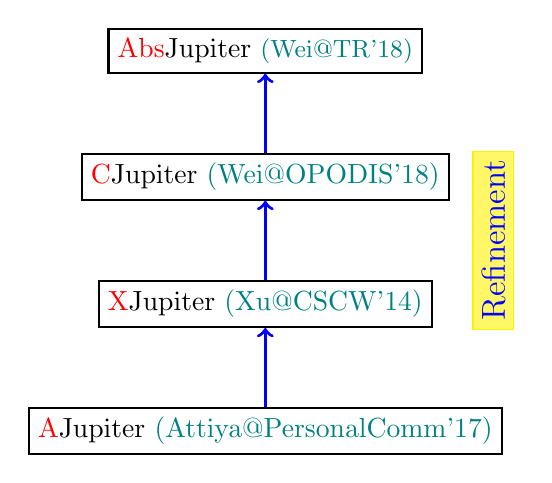
\begin{tikzpicture}[every node/.style = {draw, thick},
  node distance = 1.0cm and 2.5cm,
  every edge/.style = {->, draw, very thick, blue},
  txt/.style = {draw = none}]
  \node (absjupiter) [] {\red{Abs}Jupiter \teal{\small (Wei@TR'18)}};
  \node (cjupiter) [below = of absjupiter] {\red{C}Jupiter \teal{(Wei@OPODIS'18)}};

  \node (xjupiter) [below = of cjupiter] {\red{X}Jupiter \teal{(Xu@CSCW'14)}};
  \node (ajupiter) [below = of xjupiter] {\red{A}Jupiter \teal{(Attiya@PersonalComm'17)}};

  \path (ajupiter) edge (xjupiter)
	(xjupiter) edge node (refine) [sloped, below = 2.5cm, txt, font = \large] {\hl{\blue{Refinement}}} (cjupiter)
  	(cjupiter) edge (absjupiter);
\end{tikzpicture}
\end{document}